\section{Problem Description}

The problem resembles the Minimum Spanning Tree problem, with the addition of having to calculate the complete weight of the so-called mirror value. The mirror of an edge is the edge found when the middle of the edge list is used as a mirror. The mirror of a spanning tree is found by adding up all the mirrors of the edges in the tree. The \textsc{MirrorFriendlyMinimumSpanningTree} (MSFMST) problem deals with finding a tree where the highest value of the tree and the mirror of the tree is at most some value $B$.

%mirror edges to the edges used in the spanning tree, and finding the largest of those two values. This value has to be smaller than some given number B. \\
	
	The given problem is a graph with 3 nodes and three edges, so all nodes are connected in a cycle, as seen in \Cref{fig:example}. The problem will return true, since the spanning tree with edges $e_1$ and $e_3$ have a complete weight of 4, and the mirror edges, which are also $e_3$ and $e_1$ will have a complete weight of 4 also. If any other spanning tree is chosen, either the spanning trees complete weight or the complete weight of the mirror edges will be 5 or more.
	
	\begin{figure}[!htb]
	\centering
	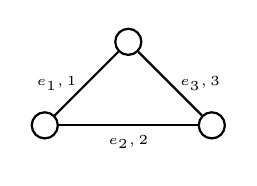
\begin{tikzpicture}[auto,node distance=1.5cm,
	  thick,main node/.style={circle,draw,font=\sffamily\tiny\bfseries}]
	
	  \node[main node] (1) {};
	  \node[main node] (2) [above right of=1] {};
	  \node[main node] (3) [below right of=2] {};
	 % \node[main node] (4) [right of=3] {4};
	
	  \path[every node/.style={font=\sffamily\tiny}]
	    (1) edge node [left] {$e_1,1$} (2)
	    	edge [right] node [below] {$e_2,2$} (3)
	    (2) edge node [right] {$e_3,3$} (3);
	    %	edge [bend left] node {0} (4)
	   % (3) edge node {$s_2$} (4);
	
	\end{tikzpicture}
	\caption{Example graph}
	\label{fig:example}
	\end{figure}

\section{MFMST $\in \mathcal{NP}$}
To show that MFMST is in $\mathcal{NP}$ we design the following polynomial time algorithm which takes a string of random values $R$ as input as well as a graph $G$.
\subsection{Algorithm}
\begin{itemize}
\item Let the string $R$ consist of index numbers for the edges in $G$: $R = r_1,r_2,\dots,r_l$.

\item If the number of edges in $R$ does not equal $n-1$, where $n$ is the number of vertices in the input graph $G$, then return NO.

\item Check whether the edges in $R$ form a tree in $G$. If not, then return NO.

\item Let the string $Q = q_1,q_2,\dots ,q_l$ consist of the mirror edges of the edges in $R$, such that if $r_1=e_k$, then $q_1=e_{m+1-k}$: . 

\item Calculate the complete weight, $W_1$, of the spanning tree formed by the edges in $R$.

\item Calculate the complete weight, $W_2$, of all the edges in $Q$.

\item If $\max \left\{W_1,W_2\right\}  \leq B$, then return YES, else return NO.\\

\end{itemize}

\subsection{Conditions}
Assume the true answer is YES

\begin{itemize}

\item There exists a spanning tree in $G$, with a total weight being less than $B$, and the total weight of the mirror edges is also less than B.

\item Construct a string of edges $R* = r_1,r_2, \dots ,r_l$ containing all the edges in the spanning tree.

\item When the algorithm receives $R*$, it will construct the spanning tree, calculate the weight of it, and calculate the weight of the mirror edges and answer YES.

\item Therefore there is a string of length $n-1$ that will return YES. The probability of creating it is positive.

\end{itemize}

Assume the true answer is NO

\begin{itemize}
\item No set of edges can create a spanning tree where both the total weight of the tree and the total weight of the mirror edges will be less than $B$.

\item If the length of $R$ is not $n-1$ then we answer NO.

\item If the length of $R$ is $n-1$, then the algorithm will check to see whether the edges in $R$ form a tree. If not then it will return NO.

\item If the edges form a spanning tree, the algorithm will calculate the complete weight of the spanning tree and the complete weight of the mirror edges.

\item Since both weights cannot be less than B, as the true answer is NO, the algorithm will return NO.\\
\end{itemize}


\subsection{Running time}
\begin{itemize}
\item We can check if there are $n-1$ edges in $R$ in time $O(n)$.

\item We can check if the edges form a tree using an algorithm like depth-first-search, in time $O(n+m)$, where $n$ is the number of nodes and $m$ is the number of edges.

\item $Q$ can be created by looping over $R$ in time $O(n)$, assuming a suitable data structure to hold edges, such as an array.

\item The total weight of $R$ is calculated in $O(n)$.

\item The total weight of $Q$ is calculated in $O(n)$.

\item The complete running time is therefore $O(n+m)$.

\end{itemize}

As we have a positive chance to answer YES when the true answer is YES, we always answer NO when the true answer is NO, and the running time of the algorithm is polynomial, we can conclude that MFMST is in $\mathcal{NP}$.